\documentclass[aspectratio=169, professionalfonts]{beamer}

\usetheme{Szeged}
\usecolortheme{dolphin}

\usepackage{amsmath, amssymb, bm}
\usepackage{tikz}
\usetikzlibrary{positioning, arrows.meta}
\usepackage{pgfplots}
\pgfplotsset{compat=1.18}

\def\R{\mathbb{R}}
\def\E{\mathbb{E}}

\definecolor{mantis}{RGB}{0, 105, 62}

\setbeamercolor{frametitle}{fg=white, bg=mantis}
\setbeamercolor{title}{fg=white, bg=mantis}
\setbeamercolor{structure}{fg=mantis}
\setbeamercolor{block title}{bg=mantis, fg=white}
\setbeamercolor{block body}{bg=mantis!10}

\title{Training Neural Networks}
\subtitle{From SGD to Scaling Laws}
\author{Lebnet Tech Fellows Program}
\date{}

\begin{document}

% ------------------------------------------------------------------
\begin{frame}
\titlepage
\end{frame}

% ------------------------------------------------------------------
\begin{frame}{Roadmap}
\tableofcontents
\end{frame}

% ==================================================================
\section{The Optimisation Problem}
% ==================================================================

% ------------------------------------------------------------------
\begin{frame}{Why Training Is Hard}

We minimise the empirical risk over parameters $\Theta$:
$$\hat{\mathcal{R}}_n(\Theta)
  = \frac{1}{n}\sum_{i=1}^{n}
    \ell\!\bigl(y_i,\, f_\Theta(\mathbf{x}_i)\bigr)$$

\bigskip

Unlike linear regression:
\begin{itemize}
  \item The loss landscape is \textbf{non-convex}
        (saddle points, local minima, flat regions).
  \item \textbf{No closed-form solution.}
  \item Parameters interact multiplicatively
        ($f_\Theta = \mathbf{W}_2\,\sigma(\mathbf{W}_1\mathbf{x})$).
  \item Permuting hidden neurons gives $m!$ equivalent minima.
\end{itemize}

\bigskip

We must rely on \textbf{iterative, gradient-based} methods.

\end{frame}

% ==================================================================
\section{SGD and Momentum}
% ==================================================================

% ------------------------------------------------------------------
\begin{frame}{Stochastic Gradient Descent}

\textbf{Full gradient:} costs $O(n)$ per step (impractical for
$n \sim 10^9$).

\bigskip

\textbf{SGD:} approximate with a random mini-batch
$\mathcal{B}_t$ of size $B$:
$$\mathbf{g}_t
  = \frac{1}{B}\sum_{i \in \mathcal{B}_t}
    \nabla_\Theta\,\ell\!\bigl(y_i,\, f_\Theta(\mathbf{x}_i)\bigr),
  \qquad
  \Theta_{t+1} = \Theta_t - \eta\,\mathbf{g}_t$$

\begin{itemize}
  \item Unbiased: $\E[\mathbf{g}_t] = \nabla\hat{\mathcal{R}}_n$
  \item Variance $\sim O(1/B)$; larger $B$ = smoother but costlier
  \item Typical $B \in [32, 4096]$ (saturate GPU parallelism)
\end{itemize}

\end{frame}

% ------------------------------------------------------------------
\begin{frame}{Momentum}

SGD oscillates in high-curvature directions. \textbf{Momentum}
smooths the trajectory:

\begin{align*}
\mathbf{v}_{t+1} &= \mu\,\mathbf{v}_t + \mathbf{g}_t \\
\Theta_{t+1} &= \Theta_t - \eta\,\mathbf{v}_{t+1}
\end{align*}

\begin{itemize}
  \item $\mu \in [0,1)$, typically $0.9$
  \item $\mathbf{v}_t$ is an exponential moving average of past gradients
  \item Consistent directions accumulate; oscillations cancel
  \item Effective step size: $\eta/(1-\mu)$
        (for $\mu=0.9$, a $10\times$ boost)
\end{itemize}

\end{frame}

% ==================================================================
\section{Adam: The Modern Workhorse}
% ==================================================================

% ------------------------------------------------------------------
\begin{frame}{Adaptive Learning Rates}

\textbf{Problem:} different parameters can have wildly different
gradient scales.

\bigskip

\textbf{Adam} (Kingma \& Ba, 2015) combines momentum with
per-parameter scaling:

\begin{align*}
\mathbf{m}_{t+1} &= \beta_1\,\mathbf{m}_t
  + (1-\beta_1)\,\mathbf{g}_t
  &&\text{(first moment)} \\[4pt]
\mathbf{v}_{t+1} &= \beta_2\,\mathbf{v}_t
  + (1-\beta_2)\,\mathbf{g}_t^2
  &&\text{(second moment)}
\end{align*}

Bias-corrected:
$\;\hat{\mathbf{m}}_t = \frac{\mathbf{m}_t}{1-\beta_1^t}$,
\quad
$\hat{\mathbf{v}}_t = \frac{\mathbf{v}_t}{1-\beta_2^t}$

\bigskip

$$\boxed{\Theta_{t+1}
  = \Theta_t
  - \eta\,\frac{\hat{\mathbf{m}}_t}
               {\sqrt{\hat{\mathbf{v}}_t}+\epsilon}}$$

Defaults: $\beta_1=0.9$, $\beta_2=0.999$, $\epsilon=10^{-8}$.

\end{frame}

% ------------------------------------------------------------------
\begin{frame}{Intuition for Adam}

The denominator $\sqrt{\hat{\mathbf{v}}_t}$ tracks the RMS
of recent gradients.

\bigskip

\begin{itemize}
  \item Parameters with \textbf{large} gradients get \textbf{smaller}
        effective learning rates.
  \item Parameters with \textbf{small} gradients get \textbf{larger}
        effective learning rates.
  \item The update magnitude is roughly
        $\eta\cdot\text{sign}(\mathbf{g})$, largely
        independent of gradient scale.
\end{itemize}

\bigskip

\begin{alertblock}{AdamW}
For neural networks, $L_2$ regularisation inside Adam gets
distorted by the adaptive denominator.
\textbf{AdamW} decouples weight decay:
$\;\Theta_{t+1} = (1-\eta\lambda)\Theta_t
  - \eta\,\frac{\hat{\mathbf{m}}_t}
               {\sqrt{\hat{\mathbf{v}}_t}+\epsilon}$
\end{alertblock}

\end{frame}

% ==================================================================
\section{Weight Initialisation}
% ==================================================================

% ------------------------------------------------------------------
\begin{frame}{Why Initialisation Matters}

For a layer $\mathbf{z} = \mathbf{W}\mathbf{h}$ with
$\mathbf{W} \in \R^{d_\text{out}\times d_\text{in}}$:

$$\text{Var}(z_i) = d_\text{in}\cdot\sigma_W^2\cdot\sigma_h^2$$

After $L$ layers the variance is
$\bigl(d_\text{in}\,\sigma_W^2\bigr)^L \sigma_x^2$.

\bigskip

\begin{itemize}
  \item $\sigma_W^2 > 1/d_\text{in}$: activations \textbf{explode}
  \item $\sigma_W^2 < 1/d_\text{in}$: activations \textbf{vanish}
\end{itemize}

\bigskip

\begin{block}{Standard Initialisations}
\begin{itemize}
  \item \textbf{Xavier} (tanh/sigmoid):
    $W_{ij} \sim \mathcal{N}\!\bigl(0,\;
      \frac{2}{d_\text{in}+d_\text{out}}\bigr)$
  \item \textbf{He} (ReLU):
    $W_{ij} \sim \mathcal{N}\!\bigl(0,\;
      \frac{2}{d_\text{in}}\bigr)$
    \quad (compensates for ReLU zeroing half the units)
\end{itemize}
\end{block}

\end{frame}

% ==================================================================
\section{Normalisation}
% ==================================================================

% ------------------------------------------------------------------
\begin{frame}{Batch Norm vs Layer Norm}

\begin{columns}[t]
\column{0.5\textwidth}
\begin{block}{Batch Normalisation}
Normalise across the \textbf{batch} at each neuron:
$$\hat{z}_i
  = \frac{z_i - \mu_\mathcal{B}}
         {\sqrt{\sigma_\mathcal{B}^2+\epsilon}}$$

$\gamma,\beta$ are learned scale/shift.

\smallskip

\begin{itemize}
  \item Prevents internal covariate shift
  \item Needs a batch; unreliable for variable-length sequences
\end{itemize}
\end{block}

\column{0.5\textwidth}
\begin{block}{Layer Normalisation}
Normalise across \textbf{features} of a single example:
$$\text{LN}(\mathbf{x})
  = \gamma\odot\frac{\mathbf{x}-\mu}{\sigma+\epsilon}+\beta$$

\smallskip

\begin{itemize}
  \item Independent of batch size
  \item Standard for transformers
  \item \textbf{RMSNorm}: drops the mean
        centering (used in LLaMA, Gemma)
\end{itemize}
\end{block}
\end{columns}

\end{frame}

% ==================================================================
\section{Regularisation}
% ==================================================================

% ------------------------------------------------------------------
\begin{frame}{Weight Decay and Dropout}

\begin{columns}[t]
\column{0.5\textwidth}
\begin{block}{Weight Decay ($L_2$)}
$$\hat{\mathcal{R}}^{\text{reg}}
  = \hat{\mathcal{R}} + \frac{\lambda}{2}\|\Theta\|_2^2$$

Update becomes:
$$\Theta_{t+1}
  = (1-\eta\lambda)\,\Theta_t
  - \eta\,\nabla\hat{\mathcal{R}}$$

Parameters shrink by $(1-\eta\lambda)$ each step.
\end{block}

\column{0.5\textwidth}
\begin{block}{Dropout}
Zero out each hidden unit with probability $p$:
$$\tilde{h}_j = \begin{cases}
  0 & \text{prob } p \\
  h_j/(1-p) & \text{prob } 1-p
\end{cases}$$

\begin{itemize}
  \item Trains an implicit ensemble of sub-networks
  \item Full network at test time $\approx$ ensemble average
\end{itemize}
\end{block}
\end{columns}

\end{frame}

% ==================================================================
\section{Learning Rate Schedules}
% ==================================================================

% ------------------------------------------------------------------
\begin{frame}{Warmup + Cosine Decay}

\begin{columns}[c]
\column{0.45\textwidth}
\begin{itemize}
  \item \textbf{Warmup} ($t \le T_w$):
    ramp linearly from $\sim\!0$ to $\eta_\text{max}$.
    Prevents large early updates before Adam stabilises.
  \item \textbf{Cosine decay} ($t > T_w$):
    $$\eta_t = \eta_\text{min}
      + \tfrac{1}{2}(\eta_\text{max}-\eta_\text{min})
        \bigl(1+\cos\tfrac{\pi(t-T_w)}{T-T_w}\bigr)$$
\end{itemize}

This is the dominant schedule for modern LLM training.

\column{0.55\textwidth}
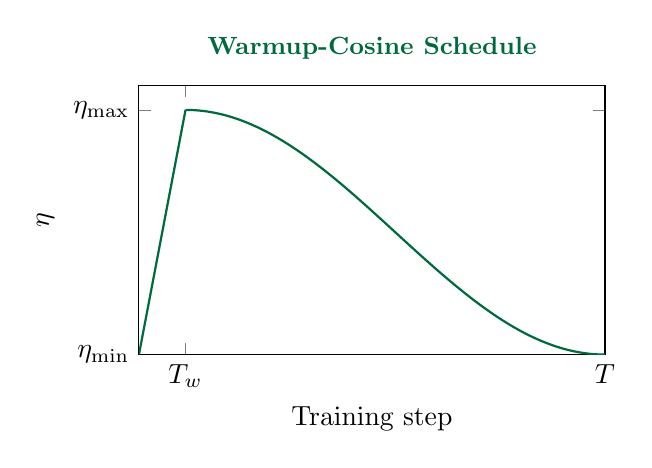
\begin{tikzpicture}
\begin{axis}[
    width=7.5cm, height=5cm,
    xlabel={Training step},
    ylabel={$\eta$},
    xmin=0, xmax=100, ymin=0, ymax=1.1,
    xtick={10,100},
    xticklabels={$T_w$,$T$},
    ytick={0,1},
    yticklabels={$\eta_\text{min}$,$\eta_\text{max}$},
    title style={font=\small\bfseries\color{mantis}},
    title={Warmup-Cosine Schedule},
]
\addplot[domain=0:10, samples=20, color=mantis, thick] {x/10};
\addplot[domain=10:100, samples=100, color=mantis, thick]
  {0.5*(1+cos(deg(pi*(x-10)/90)))};
\end{axis}
\end{tikzpicture}
\end{columns}

\end{frame}

% ==================================================================
\section{Scaling Laws}
% ==================================================================

% ------------------------------------------------------------------
\begin{frame}{Power Laws in Deep Learning}

Test loss follows \textbf{power laws} in model size $N$,
data $D$, and compute $C$:

\begin{align*}
\mathcal{L}(N) &= \left(\frac{N_c}{N}\right)^{\!\alpha_N}
  + \mathcal{L}_\infty \\[4pt]
\mathcal{L}(D) &= \left(\frac{D_c}{D}\right)^{\!\alpha_D}
  + \mathcal{L}_\infty
\end{align*}

Performance depends primarily on total compute
$C \approx 6ND$, largely independent of model shape.

\end{frame}

% ------------------------------------------------------------------
\begin{frame}{Chinchilla: Compute-Optimal Scaling}

Given a fixed compute budget $C$, how to split between
model size $N$ and training tokens $D$?

\bigskip

\begin{columns}[c]
\column{0.55\textwidth}
\begin{itemize}
  \item \textbf{Kaplan et al.\ (2020):}
    scale $N$ faster than $D$.
    Led to GPT-3 (175B params, 300B tokens).
  \item \textbf{Hoffmann et al.\ (2022, Chinchilla):}
    scale $N$ and $D$ equally.
    $$N_\text{opt} \propto C^{0.5},
      \quad D_\text{opt} \propto C^{0.5}$$
    Rule of thumb: $D \approx 20N$.
\end{itemize}

\column{0.45\textwidth}
\begin{alertblock}{Result}
Chinchilla (70B, 1.4T tokens) matched
Gopher (280B, 300B tokens) at $4\times$ lower
inference cost.
\end{alertblock}

\smallskip

Modern practice ``over-trains'' on
more tokens for smaller, cheaper-to-serve models (LLaMA).
\end{columns}

\end{frame}

% ==================================================================
\section{Post-Training}
% ==================================================================

% ------------------------------------------------------------------
\begin{frame}{From Language Model to Assistant}

Pretraining gives next-token prediction. Three steps
turn it into a helpful assistant:

\bigskip

\begin{block}{1.\ Supervised Fine-Tuning (SFT)}
Train on (prompt, response) pairs with cross-entropy
\textbf{only on the response tokens}.
Teaches format; small LR, few epochs.
\end{block}

\begin{block}{2.\ Reward Model}
Collect human preferences $\mathbf{y}_w \succ \mathbf{y}_l$.
Train $r_\phi(\mathbf{x},\mathbf{y})$ via Bradley-Terry:
$p(\mathbf{y}_w\!\succ\!\mathbf{y}_l)
  = \sigma\!\bigl(r_\phi(\mathbf{x},\mathbf{y}_w)
  - r_\phi(\mathbf{x},\mathbf{y}_l)\bigr)$
\end{block}

\begin{block}{3.\ RLHF / DPO}
Maximise expected reward while staying close to the SFT model
(KL penalty prevents reward hacking).
DPO folds the reward model into a single loss, no RL needed.
\end{block}

\end{frame}

% ==================================================================
\section{Putting It All Together}
% ==================================================================

% ------------------------------------------------------------------
\begin{frame}{The Modern Training Recipe}

\begin{center}
\small
\renewcommand{\arraystretch}{1.3}
\begin{tabular}{l l l}
\textbf{Component} & \textbf{Standard Choice} & \textbf{Why} \\[2pt]
\hline
Optimiser & AdamW &
  Adaptive LR + decoupled decay \\
Schedule & Warmup + cosine &
  Stable start, smooth decay \\
Precision & BF16 + FP32 master &
  Speed + range + update fidelity \\
Normalisation & RMSNorm (pre-norm) &
  Stable gradients, efficient \\
Initialisation & $\sim\mathcal{N}(0,1/\sqrt{d})$ &
  Variance preservation \\
Grad.\ clipping & Global norm $\le 1.0$ &
  Prevents explosion \\
Post-training & SFT $\to$ DPO / RLHF &
  Format $\to$ quality alignment
\end{tabular}
\end{center}

\end{frame}

% ------------------------------------------------------------------
\begin{frame}{Recap: The Full Story}

\begin{enumerate}
  \item \textbf{Problem:} non-convex, no closed form;
        we need iterative gradient methods.
  \item \textbf{SGD + Momentum:} cheap, unbiased gradient estimates;
        momentum smooths oscillations.
  \item \textbf{Adam:} per-parameter adaptive learning rates;
        AdamW decouples weight decay.
  \item \textbf{Initialisation:} Xavier/He keep activations stable
        across layers.
  \item \textbf{Normalisation:} BatchNorm or LayerNorm prevent
        covariate shift.
  \item \textbf{Regularisation:} weight decay and dropout
        fight overfitting.
  \item \textbf{LR schedule:} warmup + cosine is the standard
        for LLMs.
  \item \textbf{Scaling laws:} loss $\sim$ power law in $N$, $D$, $C$;
        scale model and data together.
  \item \textbf{Post-training:} SFT $\to$ RLHF/DPO turns a
        language model into an assistant.
\end{enumerate}

\end{frame}

% ------------------------------------------------------------------
{
\setbeamercolor{background canvas}{bg=mantis}
\setbeamercolor{normal text}{fg=white}
\usebeamercolor[fg]{normal text}
\begin{frame}[c]
\centering
\Huge\textbf{Questions?}
\end{frame}
}

\end{document}
